\documentclass[twocolumn]{article}
\usepackage[margin=0.75cm]{geometry}
\usepackage{hyperref}
\hypersetup{
    colorlinks,
    citecolor=blue,
    filecolor=blue,
    linkcolor=blue,
    urlcolor=blue
}

\usepackage{graphicx, multicol, wrapfig, caption, multirow, mathtools, amsfonts, booktabs, siunitx, tikz, pgfplots}
\usetikzlibrary{positioning, arrows, fit}

\setlength{\columnseprule}{.75pt}
\def\columnseprulecolor{\color{black}}
\newcommand{\overbar}[1]{\mkern 1.5mu\overline{\mkern-1.5mu#1\mkern-1.5mu}\mkern 1.5mu}

\setlength{\parindent}{0pt}
\setlength{\parskip}{6pt}

\everymath{\displaystyle}

\title{
	\vspace{-2em}
	\normalsize \textbf{ECE 240 Formula Sheet} \\
	\small Eddie Guo \\
	\dotfill
	\vspace{-5em}
}
\date{}

\begin{document}
\maketitle

\small

\textbf{Properties of Signals}

$f_e(t) \iff f(t) = f(-t)$ \hfill $f_0(t) \iff f(t) = -f(-t)$

$\int_{-a}^a f_e(t)\ dt = 2\int_0^a f_e(t)\ dt$ \hfill $\int_{-a}^a f_o(t)\ dt = 0$

$f_e(t) + f_e(t) = f_e(t)$ \hfill $f_o(t) + f_o(t) = f_o(t)$

$f_e(t) f_e(t) = f_e(t)$ \hfill $f_o(t) f_o(t) = f_e(t)$ \hfill $f_e(t) f_o(t) = f_o(t)$

$\forall f,\ \exists f(t)$ s.t. $f(t) = f_e(t) + f_o(t)$

$\quad f_e(t) = \frac{1}{2} [f(t) + f(-t)]$ \hfill $f_o(t) = \frac{1}{2}[f(t) - f(-t)]$

\dotfill

\textbf{Classifying Signals}

Energy signal: $E = \int_{-\infty}^\infty |f(t)|^2\ dt < \infty$ \hfill $|f(t)|^2 = f(t) \overline{f(t)}$

Power signal (non-periodic):  $P = \lim_{T \to \infty} \frac{1}{T} \int_{-T/2}^{T/2} |f(t)|^2\ dt$

Power signal (periodic): $P = \frac{1}{T} \int_{-T/2}^{T/2} |f(t)|^2\ dt$ \hfill $0 < P < \infty$

$f(t) = \sum_{i=1}^k A_i \cos(\omega_i t + \phi_i) \implies P = \frac{1}{2} \sum_{i=1}^k A_i^2$

If $a$ is period of $f$ and $b$ is period of $g$, period of $f+g$ is LCM($a, b$)

$\quad f(t+T) = f_1(t+k_1 T_1) + f_2(t+k_2 T_2)$ periodic iff $\frac{k_1}{k_2} = \frac{T_2}{T_1}$

$\quad T = k_1 T_1 = k_2 T_2$

\vspace{-.5em}
\dotfill

\textbf{Signal Operations}

Time reversal: $y(t) = f(-t)$

Time shift: $y(t) = f(t-b)$ \hfill $b > 0$: right, $b < 0$: left

Time scale: $y(t) = f(at)$

$\quad |a| < 1$: stretch, $|a| > 1$: compress, $|a| < 0$: reflect over y-axis

Combined ops: $y(t) = f(at-b)$

$\quad$Time shift by $b$ then scale by $a$ OR scale by $a$ then shift by $b/a$

\vspace{-.5em}
\dotfill

\textbf{Elementary Signals}

Heaviside: $H(t) = \frac{1}{2} + \frac{1}{\pi} \arctan(\lambda t)$

Unit step: $u(t) = \lim_{\lambda \to \infty} H(t) = \begin{cases} 1, & t > 0 \\ 0, & t < 0 \end{cases}$

$\quad \int_{-\infty}^t u(t-T)\ dt = \left( \int_T^t dt \right) u(t-T)$

Rectangular pulse: $p_d(t) = u(t+d/2) - u(t-d/2) = \begin{cases} 1, & |t| < d/2 \\ 0, & |t| > d/2 \end{cases}$

Unit impulse: $\delta(t) = \lim_{\sigma \to 0} \frac{dH(t)}{dt} = \frac{du(t)}{dt}, \quad \sigma = 1 / \lambda$

$\quad \int_{-\infty}^\infty \delta(t)\ dt = 1, \quad \delta (t) = 0,\ \forall t \neq 0$ \hfill $\phi(t) \delta(t-T) = \phi(T) \delta(t-T)$

$\quad$Sampling: $\int_{-\infty}^\infty \phi(t) \delta(t-T)\ dt = \int_{-\infty}^\infty \phi(t) \delta(T-t)\ dt = \phi(T)$

% $\quad$\begin{tikzpicture}
% \begin{axis}[ xlabel={$t$},
%     ymax=1.2,
%     xticklabels={,,},
%     yticklabels={,,},
%     axis x line = middle,
%     axis y line = middle,
%     width=0.4\columnwidth, ]
% \addplot[domain=-15:15, samples=100, mark size=1]{ sin(deg(x)) / x };
% \end{axis}
% \end{tikzpicture}

\newpage

$\quad \int_{-\infty}^t \delta(t-T)\ dt = u(t-T)$ \hfill $\quad \delta(at) = \frac{1}{|a|} \delta(t) \implies \delta(t) = \delta(-t)$

$\text{sinc}(t) = \frac{\sin t}{t}, \quad$ zeroes at $n \pi,\ n \in \mathbb{Z}$

Complex exponential: $f(t) = Ae^{st}, \quad s = \sigma + j \omega, A = |A| e^{j \theta}$

$\quad f(t) = |A|e^{\sigma t} \left( \cos(\omega t + \theta) + j \sin (\omega t + \theta) \right)$

$\quad \sigma < 0$: decaying sinusoid, $\sigma = 0$: sinusoid, $\sigma > 0$: growing sinusoid

\vspace{-.5em}
\dotfill

\textbf{Continuous-Time Signal Properties}

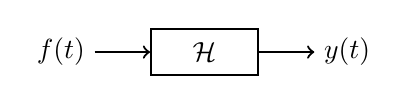
\begin{tikzpicture}
    \node (origin) at (0, 0) {$f(t)$};
    \node (H) [draw, thick, rectangle, align=center, inner xsep=1.5em, inner ysep=.5em, right=2em of origin] {$\mathcal{H}$};
    \node (y) [right=2em of H] {$y(t)$};
    \draw [->, thick] (origin) -- (H.west);
    \draw [->, thick] (H.east) -- (y);
\end{tikzpicture}
\hfill
$\mathcal{H}$ is the system

$\mathcal{H}$ is memoryless iff $y(t_0) = H[f(t_0)]$, else has memory.

$\mathcal{H}$ is causal iff $y(t_0)$ is a fn of $f(t)$ for $t < t_0$ (not future values).

$\mathcal{H}$ is linear iff $a_1 f_1 + a_2 f_2 \xrightarrow{\mathcal{H}} a_1 y_1 + a_2 y_2$. That is, given $f_1(t) \xrightarrow{\mathcal{H}} y_1(t)$ and $f_2(t) \xrightarrow{\mathcal{H}} y_2(t)$, superposition and homogeneity are satisfied.

\vspace{-.5em} $\quad$
\begin{minipage}{0.9\columnwidth}
    \begin{enumerate}
        \item Is $\frac{dy}{dt} + 2y = f^2(t)$ linear?
        \item $\frac{dy_1}{dt} + 2y_1 = f_1^2 \implies a_1 \frac{dy_1}{dt} + 2 a_1 y_1 = a_1 f_1^2$
        \item $\frac{dy_2}{dt} + 2y_2 = f_2^2 \implies a_2 \frac{dy_2}{dt} + 2 a_2 y_2 = a_2 f_2^2$
        \item $\frac{d}{dt} (a_1 y_1 + a_2 y_2) + 2(a_1 y_1 + a_2 y_2) = a_1 f_1^2 + a_2 f_2^2 \neq (a_1 f_1 + a_2 f_2)^2$ \hfill Thus, $\mathcal{H}$ is nonlinear.
    \end{enumerate}
\end{minipage}

$\mathcal{H}$ is time-invariant iff $f(t) \xrightarrow{\mathcal{H}} y(t) \implies f(t-T) \xrightarrow{\mathcal{H}} y(t-T)$

\vspace{-.5em} $\quad$
\begin{minipage}{0.9\columnwidth}
    \begin{enumerate}
        \item $\mathcal{H}: f \mapsto y,\ y = tf(t)$.
        \item Let $y_1(t) = tf_1(t)$, $y_2(t) = tf_2(t),\ \text{and } f_2(t) = f_1(t-T)$.
        \item Then $y_2(t) = t f_1(t-T)$ but $y_1(t-T) = (t-T) f_1(t-T)$.
        \item Thus, $\mathcal{H}$ is time-varying.
    \end{enumerate}
\end{minipage}

Another example:

\vspace{-.5em} $\quad$
\begin{minipage}{0.9\columnwidth}
    \begin{enumerate}
        \item $\mathcal H: f \mapsto y,\ y(t) = f(at)$.
        \item $y_1(t-T) = f_1(a(t-T)) = f_1(at - aT)$.
        \item $f_2(t) = f_1(t-T) \implies y_2(t) = y_1(at - T)$.
        \item Thus, $\mathcal{H}$ is time-varying.
    \end{enumerate}
\end{minipage}

$\mathcal{H}$ is BIBO stable iff $|f(t)| \leq A < \infty \implies |y(t)| \leq B < \infty,\ A, B \in \mathbb{R}$.

\vspace{-.5em}
\dotfill

\textbf{Convolutions}

Convolution: $f_1(t) * f_2(t) = \int_{-\infty}^\infty f_1(\tau) f_2(t-\tau)\ d\tau$

If $h(t) = \mathcal{H}(\delta(t))$, then $y(t) = \mathcal{H}(f(t)) = f(t) * h(t)$. That is,

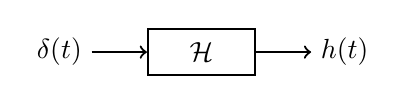
\begin{tikzpicture}
    \node (origin) at (0, 0) {$\delta(t)$};
    \node (H) [draw, thick, rectangle, align=center, inner xsep=1.5em, inner ysep=.5em, right=2em of origin] {$\mathcal{H}$};
    \node (y) [right=2em of H] {$h(t)$};
    \draw [->, thick] (origin) -- (H.west);
    \draw [->, thick] (H.east) -- (y);
\end{tikzpicture}
\hfill
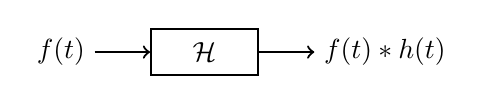
\begin{tikzpicture}
    \node (origin) at (0, 0) {$f(t)$};
    \node (H) [draw, thick, rectangle, align=center, inner xsep=1.5em, inner ysep=.5em, right=2em of origin] {$\mathcal{H}$};
    \node (y) [right=2em of H] {$f(t) * h(t)$};
    \draw [->, thick] (origin) -- (H.west);
    \draw [->, thick] (H.east) -- (y);
\end{tikzpicture}

Commutation: $f_1(t)*f_2(t) = f_2(t)*f_1(t)$

Distribution: $f_1*(f_2+f_3) = f_1*f_2 + f_1*f_3$

Association: $f_1*(f_2*f_3) = (f_1*f_2)*f_3$

Time shifting: $f_1(t-T_2)*f_2(t-T_2) = y(t-T_1-T_2)$

$\quad f_1(t-T) * f_2(t) = y(t-T)$ \hfill $f_1(t) * f_2(t-T) = y(t-T)$

Convolution w/ unit impulse: $f(t) * \delta(t) = f(t)$

Causal signals: $f_1(t) * f_2(t) = \int_0^t f_1(\tau) f_2(t-\tau)\ d\tau$


\cleardoublepage


\textbf{LTI System Properties}

$\mathcal{H}$ is memoryless iff $h(t) = k \delta(t)$.

$\mathcal{H}$ is causal iff $h(t) = 0\ \forall t < 0$.

$\mathcal{H}$ is is BIBO stable iff $h(t)$ is absolutely integrable, i.e.,

$\quad \int_{-\infty}^\infty |h(t)|\ dt \leq M < \infty$

\dotfill

\textbf{Inner Products \& Orthogonality}

Inner product: $\langle f_1, f_2 \rangle = \int_{t_1}^{t_2} f_1(t) \overline{f_2(t)}\ dt$

$\quad$Orthogonal over $[t_1, t_2] \iff \langle f_1, f_2 \rangle = 0$

$\quad$Orthogonal set if $f_1, \dots, f_n$ over $[t_1, t_2]$ is $\langle f_i, f_j \rangle = \begin{cases} 0, & i \neq j \\ E_{ij}, & i = j \end{cases}$

Let $\mathcal{S} = \{ 1, \cos \omega_0 t, \dots, \cos n \omega_t, \dots, \sin \omega_0 t, \dots, \sin n \omega_t, \dots \}$. Then $\mathcal{S}$ is an orthognal set over the interval $[-T/2, T/2]$ iff

\vspace{-.5em}\begin{enumerate}
    \item $\langle \cos n \omega_0 t, \sin k \omega_0 t \rangle = \begin{cases} 0, & n \neq k \\ T/2, & n = k \neq 0 \end{cases}$
    \item $\langle \sin n \omega_0 t, \sin k \omega_0 t \rangle = \begin{cases} 0, & n \neq k \\ T/2, & n = k \neq 0 \end{cases}$
    \item $\langle 1, \sin n \omega_0 t \rangle = 0, \quad \forall n$
    \item $\langle 1, \cos n \omega_0 t \rangle = 0, \quad \forall n$
\end{enumerate} \vspace{-.5em}

\vspace{-.5em}
\dotfill

\textbf{Trigonometric Fourier Series}

$f(t) = f(t+T) \implies f(t) = a_0 + \sum_{n=1}^\infty \left( a_n \cos n \omega_0 t + b_n \sin n \omega_0 t \right)$

$\quad a_0 = \frac{1}{T} \int_{-T/2}^{T/2} f(t)\ dt$ \hfill $\omega_0 = \frac{2\pi}{T}$

$\quad a_n = \frac{2}{T} \int_{-T/2}^{T/2} f(t) \cos n \omega_0 t\ dt$ \hfill $b_n = \frac{2}{T} \int_{-T/2}^{T/2} f(t) \sin n \omega_0 t\ dt$

$\quad f(t) \text{ odd } \implies a_0 = a_n = 0$ \hfill $b_n = \frac{4}{T} \int_0^{T/2} f(t) \sin n \omega_0 t\ dt$

$\quad f(t) \text{ even } \implies b_n = 0$ \hfill $a_n = \frac{4}{T} \int_0^{T/2} f(t) \cos n \omega_0 t\ dt$

Let $f(t) = f(t+T)$ and $S_k(t) = a_0 + \sum_{n=1}^k (a_0 \cos n \omega_0 t + b_n \sin n \omega_0 t)$. Then if $\epsilon_k(t) = f(t) - S_k(t)$,

$\quad P_{\epsilon_k}(t) = \frac{1}{T} \int_{-T/2}^{T/2} \epsilon_k^2(t)\ dt = \frac{1}{T} \int_{-T/2}^{T/2} f^2(t)\ dt - a_0^2 - \frac{1}{2} \sum_{n=1}^k (a_n^2 + b_n^2)$

$\quad \frac{1}{T} \int_{-T/2}^{T/2} f^2(t)\ dt \geq a_0^2 + \frac{1}{2} \sum_{n=1}^k (a_n^2 + b_n^2)$ \hfill $\lim_{n \to \infty} a_n = \lim_{n \to \infty} b_n = 0$

If $\int_T |f(t)|\ dt < \infty$ and $f$ has finite number of maxima, minima, discontinuities in each period, then the series converges to $f(t)$ except at discontinuities, where it converges to $\frac{1}{2} [f(t_d^-) + f(t_d^+)]$.

\dotfill

\textit{Compact Form}

$f(t) = c_0 + \sum_{n=1}^\infty c_n \cos(n \omega_0 t + \theta_n)$

$c_0 = a_0$ \hfill $c_n = \sqrt{a_n^2 + b_n^2}$ \hfill $\theta_n = \arctan(-b_n/a_n),\ \theta_n \in [-\pi, \pi]$

\newpage

\textit{Exponential Form}

$f(t) = \sum_{n=-\infty}^\infty D_n e^{jn\omega_0t}$

$\quad D_n = \frac{a_n - jb_n}{2}$ \hfill $D_{-n} = \frac{a_n + jb_n}{2}$ \hfill $D_0 = a_0$

$\quad D_n = \frac{1}{T} \int_T f(t) e^{-j n \omega_0 t}\ dt$ \hfill $D_n = \frac{c_n}{2} e^{j \theta_n}, \quad D_{-n} = \frac{c_n}{2} e^{-j \theta_n}$

$|D_n| = \frac{c_n}{2} \implies$ even fn \hfill $\angle D_n = \theta_n, \quad D_{-n} = -\theta_n \implies$ odd fn

$f(t)$ even: $|D_n| = \frac{|a_n|}{2}, \quad \angle D_n = \begin{cases} 0, & a_n > 0 \\ \pm \pi, & a_n < 0 \end{cases}$

$f(t)$ odd: $|D_n| = \frac{|b_n|}{2}, \quad \angle D_n = \begin{cases} \pi/2, & b_n > 0 \\ -\pi/2, & b_n < 0 \end{cases}$

\dotfill

\textit{Parseval's Theorem (Discrete)}

$P_f = a_0^2 + \frac{1}{2} \sum_{n=1}^\infty (a_n^2 + b_n^2) = c_0^2 + \frac{1}{2} \sum_{n=1}^\infty c_n^2 = D_0^2 + 2 \sum_{n=1}^\infty |D_n|^2 = \sum_{n=-\infty}^\infty |D_n|^2$ \hfill $P_{f_k}$ is power of FS w/ $k$ terms

Error to $n$\%: $P_{f_k} = (1-n\%) P_f$ \hfill \textbf{Caution:} Count the const term!

\vspace{-.5em}
\dotfill

\textbf{Identities}

$\sin(x \pm y) = \sin x \cos y \pm \cos x \sin y$ \hfill $e^{j\theta} = \cos \theta + j \sin \theta$

$\cos(x \pm y) = \cos x \cos y \mp \sin x \sin y$ \hfill $\cos \theta = \frac{e^{j\theta} + e^{-j\theta}}{2}$

$\sin \mapsto \cos:\ \sin \theta = \cos\left(\theta - \SI{90}{\degree}\right)$ \hfill $\sin \theta = \frac{e^{j\theta} - e^{-j\theta}}{2j}$

$\cos \mapsto \sin:\ \cos \theta = \sin\left(\theta + \SI{90}{\degree}\right)$

\vspace{-.5em}
\dotfill

\textit{Double Angle Formulas}

$\sin x + \sin y = 2 \sin \left( \frac{x+y}{2} \right) \cos \left( \frac{x-y}{2} \right)$

$\sin x - \sin y = 2 \cos \left( \frac{x+y}{2} \right) \sin \left( \frac{x-y}{2} \right)$

$\cos x + \cos y = 2 \cos \left( \frac{x+y}{2} \right) \cos \left( \frac{x-y}{2} \right)$

$\cos x - \cos y = -2 \sin \left( \frac{x+y}{2} \right) \sin \left( \frac{x-y}{2} \right)$

\dotfill

\textit{Half Angle Formulas}

$\sin x \sin y = \frac{1}{2} [\cos(x-y) - \cos(x+y)]$

$\cos x \cos y = \frac{1}{2} [\cos(x-y) + \cos(x+y)]$

$\sin x \cos y = \frac{1}{2} [\sin(x+y) + \sin(x-y)]$

$\cos x \sin y = \frac{1}{2} [\sin(x+y) - \sin(x-y)]$

\dotfill

\textbf{Fourier Transform}

$F(\omega) = \mathcal{F} \{ f(t) \} = \int_{-\infty}^\infty f(t) e^{-j \omega t}\ dt$

$f(t) = \mathcal{F}^{-1} \{ \mathcal{F}(\omega) \} = \frac{1}{2\pi} \int_{-\infty}^\infty F(\omega) e^{j \omega t}\ d\omega$

$\mathcal{F}(\omega) = \text{Re} \{F(\omega)\} + j \text{Im}\{F(\omega)\}$ \hfill $|\mathcal{F}(\omega)|$ even, $\angle \mathcal{F}(\omega)$ odd

\dotfill

\textbf{Frequency Response of LTI Systems}

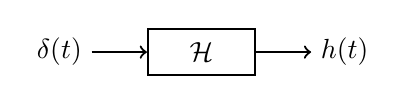
\begin{tikzpicture}
    \node (origin) at (0, 0) {$\delta(t)$};
    \node (H) [draw, thick, rectangle, align=center, inner xsep=1.5em, inner ysep=.5em, right=2em of origin] {$\mathcal{H}$};
    \node (y) [right=2em of H] {$h(t)$};
    \draw [->, thick] (origin) -- (H.west);
    \draw [->, thick] (H.east) -- (y);
\end{tikzpicture}
\hfill
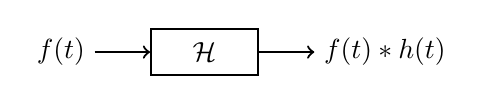
\begin{tikzpicture}
    \node (origin) at (0, 0) {$f(t)$};
    \node (H) [draw, thick, rectangle, align=center, inner xsep=1.5em, inner ysep=.5em, right=2em of origin] {$\mathcal{H}$};
    \node (y) [right=2em of H] {$f(t) * h(t)$};
    \draw [->, thick] (origin) -- (H.west);
    \draw [->, thick] (H.east) -- (y);
\end{tikzpicture}

Freq response: $H(\omega) = \frac{Y(\omega)}{F(\omega)}$

$|Y(\omega)| = |H(\omega)| |F(\omega)|$ \hfill $\angle Y(\omega) = \angle H(\omega) + \angle F(\omega)$

$\mathcal{H}$ is distortion-free if $H(\omega) = K e^{-j\omega t_0}$

\vspace{-.5em}
\dotfill

\textit{Parseval's Theorem (Continuous)}

$E_f = \int_{-\infty}^\infty |f(t)|^2\ dt = \frac{1}{2\pi} \int_{-\infty}^\infty |F(\omega)|^2\ d\omega$

E spectral density: $|F(\omega)|^2$

$\quad$Time compression $\iff$ spectral expansion

$\quad$Time expansion $\iff$ spectral compression

LPF: $|H(\omega)| = \begin{cases} e^{-j\omega t_0}, & |\omega| < \omega_c \\ 0, & |\omega| > \omega_c \end{cases}$ \hfill $|H(\omega)| = \begin{cases} 1, & |\omega| < \omega_c \\ 0, & |\omega| > \omega_c \end{cases}$

\dotfill

\textit{Impulse Response}

$Y(s) = H(s) X(s)$

$\quad x(t) = \delta(t) \implies \mathcal{L}[\delta(t)] = 1 \implies y(t) = \mathcal{L}^{-1}[H(s)] = h(t)$

$\quad$Given $h(t)$, $y(t) = \mathcal{L}^{-1} [\ \mathcal{L}[h(t)] \mathcal{L}[x(t)]\ ]$

\vspace{-.5em}
\dotfill

\textbf{Amplitude Modulation}

\textit{AM Transmission}

$\mathcal{F} \{ f(t) \cos \omega_0 t \} = \frac{1}{2} \left[ F(\omega + \omega_0) + F(\omega - \omega_0) \right]$

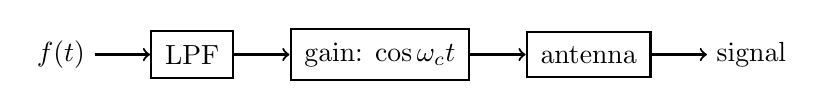
\begin{tikzpicture}
    \node (origin) at (0, 0) {$f(t)$};
    \node (lpf) [draw, thick, rectangle, align=center, inner xsep=.5em, inner ysep=.5em, right=2em of origin] {LPF};
    \node (gain) [draw, thick, rectangle, align=center, inner xsep=.5em, inner ysep=.5em, right=2em of lpf] {gain: $\cos \omega_c t$};
    \node (antenna) [draw, thick, rectangle, align=center, inner xsep=.5em, inner ysep=.5em, right=2em of gain] {antenna};
    \node (f) [right=2em of antenna] {signal};

    \draw [->, thick] (origin) -- (lpf.west);
    \draw [->, thick] (lpf.east) -- (gain.west);
    \draw [->, thick] (gain.east) -- (antenna.west);
    \draw [->, thick] (antenna.east) -- (f.west);
\end{tikzpicture}

\vspace{-.5em}
\dotfill

\textit{AM Reception}

$\mathcal{F} \{ f(t) \cos^2 \omega_0 t \} = \frac{1}{2} F(\omega) + \frac{1}{4} \left[ F(\omega + 2\omega_0) + F(\omega - 2\omega_0) \right]$

BPF selects the carrier frequency $\omega_c$ and LPF removes the $F/4$ terms.

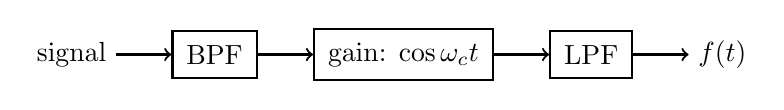
\begin{tikzpicture}
    \node (origin) at (0, 0) {signal};
    \node (lpf) [draw, thick, rectangle, align=center, inner xsep=.5em, inner ysep=.5em, right=2em of origin] {BPF};
    \node (gain) [draw, thick, rectangle, align=center, inner xsep=.5em, inner ysep=.5em, right=2em of lpf] {gain: $\cos \omega_c t$};
    \node (antenna) [draw, thick, rectangle, align=center, inner xsep=.5em, inner ysep=.5em, right=2em of gain] {LPF};
    \node (f) [right=2em of antenna] {$f(t)$};

    \draw [->, thick] (origin) -- (lpf.west);
    \draw [->, thick] (lpf.east) -- (gain.west);
    \draw [->, thick] (gain.east) -- (antenna.west);
    \draw [->, thick] (antenna.east) -- (f.west);
\end{tikzpicture}

\vspace{-.5em}
\dotfill

\textbf{Unilateral Laplace Transform}

$F(s) = \int_{0^-}^\infty f(t)e^{-st}\ dt$ \hfill $f(t)$ causal

$f(t) = \frac{1}{2 \pi j} \int_{c-j\infty}^{c+j\infty} F(s)e^{st}\ dt$

LT exists if $|f(t)| \leq M e^{\sigma_0 t},\ \sigma_0 \in \mathbb{R}$

IVT: $f(0^+) = \lim_{s \to \infty} sF(s)$ \hfill FVT: $\lim_{t \to \infty} f(t) = \lim_{s \to 0} sF(s)$

\vspace{-.5em}
\dotfill

\textit{Partial Fraction Expansion}

Real \& distinct roots: $\frac{P(s)}{Q(s)} = \frac{K_1}{s+p_1} + \cdots + \frac{K_j}{s+p_j} + \cdots + \frac{K_n}{s + p_n}$

$\quad K_j = \frac{P(s)}{Q(s)} (s+p_j) |_{s=-p_j}$

$\quad \mathcal{L}^{-1} \left[  \frac{P(s)}{Q(s)}\right] = u(t) \left( K_1 e^{-p_1 t} + \cdots + K_j e^{-p_j t} + \cdots + K_n e^{-p_n t} \right)$

Distinct complex roots: $\frac{P(s)}{Q(s)} = \frac{K}{s + (\alpha - j\beta)} + \frac{K^*}{s + (\alpha + j\beta)} + \cdots$

$\quad K = \frac{P(s)}{Q(s)} (s + \alpha - j\beta) |_{s=-(\alpha - j\beta)} = |K| \angle \theta_K$

$\quad \mathcal{L}^{-1} \left[ \frac{P(s)}{Q(s)} \right] = u(t) \left[ 2|K| e^{-\alpha t} \cos(\beta t + \theta_K) + \cdots \right]$

Repeated real roots: $\frac{P(s)}{Q(s)} = \frac{K_1}{(s+p)^n} + \frac{K_2}{(s+p)^{n-1}} + \cdots + \frac{K_n}{s+p}$

$\quad K_j = \frac{1}{(j-1)!} \left[ \frac{d^{(j-1)}}{ds^{(j-1)}} (s+p)^n F(s) \right]_{s=-p}$

\dotfill


\textbf{Zero-Input \& Zero-State Response}

$Q(s)Y(s) - N(s) = P(s) F(s) \implies Y(s) = \underbrace{\frac{N(s)}{Q(s)}}_{\text{ICs}} + \underbrace{\frac{P(s)}{Q(s)} F(s)}_{\text{forcing fn}}$

ZIR: $y_0(t) = \mathcal{L}^{-1} \left\{ \frac{N(s)}{Q(s)} \right\}$ \hfill set input $f(t) = 0$

ZSR: $y_f(t) = \mathcal{L}^{-1} \left\{ \frac{P(s)}{Q(s)} F(s) \right\}$ \hfill set ICs to 0

Use $Y(s) = H(s) F(s)$ to find the sys ODE

\vspace{-.5em}
\dotfill

\textit{BIBO Stability of LTI Systems}

$H(s) = \frac{P(s)}{Q(s)} = \beta_n + \frac{b_{n-1}s^{n-1} + \cdots + b_0}{s^n + a_{n-1} s^{n-1} + \cdots + a_0}$

$\mathcal{H}$ is BIBO stable iff all poles of $H(s)$ have a -ve real part.

If poles of a LTI sys has a -ve real part, then $h(t) = \mathcal{L}^{-1} \{ H(s) \}$ admits a FT $H(j\omega) = \mathcal{F}\{h(t)\}$. Moreover, $H(j\omega) = H(s) |_{s=j\omega}$.

\dotfill

\textbf{Block Diagrams}

\textit{Cascading Combination}

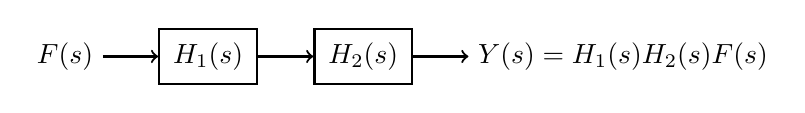
\begin{tikzpicture}
    \node (origin) at (0, 0) {$F(s)$};
    \node (H1) [draw, thick, rectangle, align=center, inner xsep=.5em, inner ysep=.5em, right=2em of origin] {$H_1(s)$};
    \node (H2) [draw, thick, rectangle, align=center, inner xsep=.5em, inner ysep=.5em, right=2em of H1] {$H_2(s)$};
    \node (y) [right=2em of H2] {$Y(s) = H_1(s) H_2(s) F(s)$};
    \draw [->, thick] (origin) -- (H1.west);
    \draw [->, thick] (H1.east) -- (H2.west);
    \draw [->, thick] (H2.east) -- (y);
\end{tikzpicture}

$H(s) = H_1(s) H_2(s)$

\vspace{-.5em}
\dotfill

\textit{Sum Combination}

\begin{minipage}{0.64\columnwidth}
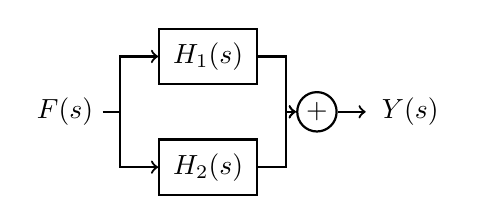
\begin{tikzpicture}
    \node (origin) at (0, 0) {$F(s)$};
    \node (H1) [draw, thick, rectangle, align=center, inner xsep=.5em, inner ysep=.5em, right=2em of origin, yshift=2em] {$H_1(s)$};
    \node (H2) [draw, thick, rectangle, align=center, inner xsep=.5em, inner ysep=.5em, right=2em of origin, yshift=-2em] {$H_2(s)$};
    \draw[black, thick] (3.2, 0) circle (0.25) node (plus) {+};
    \node (y) [circle, right=1em of plus] {$Y(s)$};


    \draw [->, thick] (origin) -- ++(2em, 0) |- (H1.west);
    \draw [->, thick] (origin) -- ++(2em, 0) |- (H2.west);
    \draw [->, thick] (H1.east) -- ++(1em, 0) |- (plus);
    \draw [->, thick] (H2.east) -- ++(1em, 0) |- (plus);
    \draw [->, thick] (plus) -- (y);
\end{tikzpicture}
\end{minipage}
\hfill
\begin{minipage}{0.35\columnwidth}
    $Y(s) = H(s) F(s)$ \\[1em]
    $H(s) = H_1(s) + H_2(s)$
\end{minipage}

\dotfill

\textit{Feedback Combination}

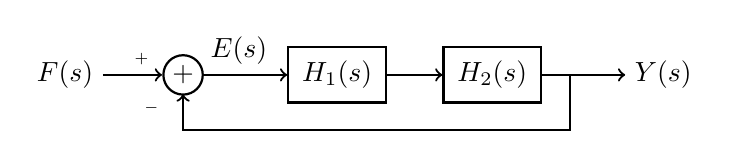
\begin{tikzpicture}
    \node (origin) at (0, 0) {$F(s)$};
    \draw[black, thick] (1.5, 0) circle (0.25) node (plus) {+};
    \node (H1) [draw, thick, rectangle, align=center, inner xsep=.5em, inner ysep=.5em, right=3em of plus] {$H_1(s)$};
    \node (H2) [draw, thick, rectangle, align=center, inner xsep=.5em, inner ysep=.5em, right=2em of H1] {$H_2(s)$};
    \node (y) [right=3em of H2] {$Y(s)$};

    \draw [->, thick] (origin) -- (plus) node [above, xshift=-1.5em] {\tiny +};
    \draw [->, thick] (plus) -- (H1.west) node[above, xshift=-1.75em] {$E(s)$};
    \draw [->, thick] (H1.east) -- (H2.west);
    \draw [->, thick] (H2.east) -- (y);
    \draw [->, thick] (H2.east) ++(1em, 0) -- ++(0, -2em) -| (plus.south)  node [left, xshift=-0.5em, yshift=-.5em] {\tiny $-$};
\end{tikzpicture} \vspace{1em}

$E(s) = F(s) - Y(s)$

$Y(s) = E(s) H_1(s) H_2(s) = [F(s) - Y(s)] H_1(s) H_2(s)$

$Y(s) = \frac{H_1(s) H_2(s)}{1+H_1(s)H_2(s)} F(s)$


% new page
\cleardoublepage


\onecolumn

\begin{table}[h!]
    \centering
    \textit{FT Properties} \\[1em]

    \begin{tabular}{lll}
        \toprule
        Operation & Time domain & Freq domain \\
        \midrule
        Linearity & $a_1 f_1(t) + a_2 f_2(t)$ & $a_1 F_1(\omega) + a_2 F_2(\omega)$ \\[0.5em]
        Symmetry & $F(t)$ & $2\pi f(-\omega)$ \\[0.5em]
        Scaling & $f(at)$ & $\frac{1}{|a|} F \left( \frac{\omega}{a} \right)$ \\[1.25em]
        Time shift & $f(t-t_0)$ & $F(\omega) e^{-j\omega t_0}$ \\[0.5em]
        Freq shift & $f(t) e^{j \omega_0 t}$ & $F(\omega - \omega_0)$ \\[0.5em]
        Time convolution & $f_1(t) * f_2(t)$ & $F_1(\omega) F_2(\omega)$ \\[0.5em]
        Freq convolution & $f_1(t) f_2(t)$ & $\frac{1}{2\pi} F_1(\omega) * F_2(\omega)$ \\[0.5em]
        Time differentiation & $\frac{d^n f}{dt^n}$ & $(j\omega)^n F(\omega)$ \\[1em]
        Time integration & $\int_{-\infty}^t f(x)\ dx$ & $\frac{F(\omega)}{j\omega} + \pi F(0) \delta(\omega)$ \\[1em]
        Periodic signal & $f(t) = f(t+T)$ & $2\pi \sum_{n=-\infty}^\infty D_n \delta(\omega - n\omega_0)$ \\[1em]
        \bottomrule
    \end{tabular}
\end{table}

\textit{Symmetry/duality:} $\mathcal{F} \{ F(t) \} = 2\pi f(-\omega)$

\textit{Symmetry example:} Find $f(t) = \mathcal{F}^{-1} \{ F(\omega) * \delta(\omega-\omega_0) \}$ if $F(\omega) = \text{rect}\left(\frac{\omega}{d}\right)$.

\vspace{-.5em}\begin{enumerate}
    \item $F(\omega) * \delta(\omega - \omega_0) = \int_{-\infty}^\infty F(\tau) \delta(\omega - \omega_0 - \tau)\ d\tau = F(\omega - \omega_0)$
    \item Recall $F(t) = 2\pi f(-\omega) \implies \mathcal{F} \{d \text{sinc} \left( \frac{td}{2} \right) \} = 2\pi \text{rect}\left(-\frac{\omega}{d}\right) = 2\pi \text{rect}\left(\frac{\omega}{d}\right)$.
    \item Also recall $\mathcal{F}^{-1} \{F(\omega - \omega_0)\} = f(t) e^{j \omega_0 t} \implies \mathcal{F}^{-1} \{\text{rect}\left(\frac{\omega-\omega_0}{d}\right)\} = \frac{d}{2\pi} \text{sinc}\left(\frac{td}{2}\right) e^{j\omega_0 t}$
\end{enumerate}

\vspace{-.5em}
\dotfill

\begin{table*}[h!]
    \centering
    \textit{FT of Important Functions} \\[1em]

    \begin{tabular}{c| cc |c| cc}
        \toprule
        & $f(t)$ & $F(\omega)$ & & $f(t)$ & $F(\omega)$ \\
        \midrule
        1 & $\delta(t)$ & 1 & 10 & $e^{j \omega_0}$ & $2\pi\delta(\omega-\omega_0)$ \\[1em]
        2 & 1 & $2\pi\delta(\omega)$ & 11 & $\cos \omega_0 t$ & $\pi [\delta(\omega-\omega_0) + \delta(\omega+\omega_0)]$ \\[1em]
        3 & $u(t)$ & $\pi \delta(\omega) + \frac{1}{j\omega}$ & 12 & $\sin \omega_0 t$ & $j\pi[\delta(\omega+\omega_0) - \delta(\omega-\omega_0)]$ \\[1em]
        4 & $\text{sgn}\ t$ & $\frac{2}{j\omega}$ & 13 & $\cos \omega_0 t\ u(t)$ & $\frac{\pi}{2} [\delta(\omega-\omega_0) + \delta(\omega+\omega_0)] + \frac{j\omega}{\omega_0^2 - \omega^2}$ \\[1em]
        5 & $e^{-at} u(t),\ a > 0$ & $\frac{1}{a + j\omega}$ & 14 & $\sin \omega_0 t\ u(t)$ & $\frac{\pi}{2j} [\delta(\omega-\omega_0) - \delta(\omega+\omega_0)] + \frac{\omega_0}{\omega_0^2 - \omega^2}$ \\[1em]
        6 & $e^{at} u(-t),\ a > 0$ & $\frac{1}{a-j\omega}$ & 15 & $e^{-at} \cos \omega_0 t\ u(t),\ a > 0$ & $\frac{a + j\omega}{(a + j\omega)^2 + \omega_0^2}$ \\[1em]
        7 & $te^{-at} u(t),\ a > 0$ & $\frac{1}{(a+j\omega)^2}$ & 16 & $e^{-at} \sin \omega_0 t\ u(t),\ a > 0$ & $\frac{\omega_0}{(a+j\omega)^2 + \omega_0^2}$ \\[1em]
        8 & $t^n e^{-at} u(t),\ a > 0$ & $\frac{n!}{(a+j\omega)^{n+1}}$ & 17 & $\text{rect}(t/d)$ & $d\ \text{sinc} \frac{\omega d}{2}$ \\[1em]
        9 & $e^{-a|t|},\ a > 0$ & $\frac{2a}{a^2 + \omega^2}$ & \\[1em]
        \bottomrule
    \end{tabular}
\end{table*}

$\mathcal{F} \{ f(t) \cos \omega_0 t \} = \frac{1}{2} \left[ F(\omega + \omega_0) + F(\omega - \omega_0)) \right]$ \hfill $\mathcal{F} \{ f(t) \cos^2 \omega_0 t \} = \frac{1}{2} F(\omega) + \frac{1}{4} \left[ F(\omega + 2\omega_0) + F(\omega - 2\omega_0) \right]$


\cleardoublepage


\begin{table}[h!]
    \centering
    \textit{LT Properties} \\[1em]

    \begin{tabular}{lll}
        \toprule
        Operation & Time domain & Laplace domain \\
        \midrule
        Scaling & $f(at),\quad a \geq 0$ & $\frac{1}{a} F\left(\frac{s}{a}\right)$ \\[1em]
        Time convolution & $f_1(t) * f_2(t)$ & $F_1(s) F_2(s)$ \\[1em]
        Time differentiation & $\frac{df}{dt}$ & $sF(s) - f(0^-)$ \\[1em]
        & $\frac{d^2 f}{dt^2}$ & $s^2 F(s) - sf(0^-) - f'(0^-)$ \\[1em]
        & $\frac{d^3 f}{dt^3}$ & $s^3 F(s) - s^2 f(0^-) - sf'(0^-) - f''(0^-)$ \\[1em]
        Time integration & $\int_{0^-}^t f(x)\ dx$ & $\frac{1}{s} F(s)$ \\[1.5em]
        & $\int_{-\infty}^t f(x)\ dx$ & $\frac{1}{s} F(s) + \frac{1}{s} \int_{-\infty}^{0^-} f(t)\ dt$ \\[1.5em]
        Time shift & $f(t-t_0) u(t-t_0)$ & $F(s)e^{-st_0},\quad t_0 \geq 0$ \\[1em]
        Frequency shift & $f(t)e^{s_0t}$ & $F(s-s_0)$ \\[1em]
        Frequency differentiation & $-tf(t)$ & $\frac{dF(s)}{ds}$ \\[1em]
        Initial value thm & $f(0^+)$ & $\lim_{s\to\infty} sF(s)$ \\[1em]
        Final value thm & $\lim_{t\to\infty} f(t)$ & $\lim_{s\to 0} sF(s)$ \\[1em]
        & & (poles of $sF(s)$ in LHP) \\[1em]
        Scale \& shift & $f(at-b)$ & $\frac{e^{-bs/a}}{a} F \left( \frac{s}{a} \right)$ \\[1em]
        \bottomrule
    \end{tabular}
\end{table} \vspace{-.5em}

\dotfill


\begin{table*}[h!]
    \centering
    \textit{Unilateral LT of Important Functions} \\[1em]

    \begin{tabular}{c| cc |c| cc}
        \toprule
        & $f(t)$ & $F(s)$ & & $f(t)$ & $F(s)$ \\
        \midrule
        1 & $\delta(t)$ & 1 & 7 & $t^n e^{\lambda t} u(t)$ & $\frac{n!}{(s-\lambda)^{n+1}}$ \\[1em]
        2 & $u(t)$ & $\frac{1}{s}$ & 8 & $\cos(bt) u(t)$ & $\frac{s}{s^2 + b^2}$ \\[1em]
        3 & $tu(t)$ & $\frac{1}{s^2}$ & 9 & $\sin(bt) u(t)$ & $\frac{b}{s^2+b^2}$ \\[1em]
        4 & $t^n u(t)$ & $\frac{n!}{s^{n+1}}$ & 10 & $e^{-at} \cos(bt) u(t)$ & $\frac{s+a}{(s+a)^2 + b^2}$ \\[1em]
        5 & $e^{\lambda t} u(t)$ & $\frac{1}{s-\lambda}$ & 11 & $e^{-at} \sin(bt) u(t)$ & $\frac{b}{(s+a)^2 + b^2}$ \\[1em]
        6 & $t e^{\lambda t} u(t)$ & $\frac{1}{(s-\lambda)^2}$ & \\[1em]
        \bottomrule
    \end{tabular}
\end{table*}



\end{document}
